\documentclass[12pt]{article}

\usepackage[utf8]{inputenc}
\usepackage{amsmath}
\usepackage{amssymb}
\usepackage{anysize}
\usepackage{color}
\usepackage{xcolor}
\usepackage{graphicx}
\usepackage{float}
\usepackage{lipsum}
\usepackage{graphicx}
\usepackage{caption}
\usepackage{subcaption}

\usepackage{listings}
\usepackage{color} %red, green, blue, yellow, cyan, magenta, black, white
\definecolor{mygreen}{RGB}{28,172,0} % color values Red, Green, Blue
\definecolor{mylilas}{RGB}{170,55,241}



\usepackage{listings}
\lstset{
	language=C++,                	% choose the language of the code
	basicstyle=\footnotesize,       % the size of the fonts that are used for the code
	numbers= left,                 	% where to put the line-numbers
	numberstyle=\footnotesize,      % the size of the fonts that are used for the line-numbers
	stepnumber=1,                   % the step between two line-numbers. If it is 1 each line will be numbered
	numbersep=5pt,                  % how far the line-numbers are from the code
	backgroundcolor=\color{white},  % choose the background color. You must add \usepackage{color}
	showspaces=false,               % show spaces adding particular underscores
	showstringspaces=false,         % underline spaces within strings
	showtabs=false,                 % show tabs within strings adding particular underscores
	frame=single,           		% adds a frame around the code
	tabsize=2,          			% sets default tabsize to 2 spaces
	captionpos=t,          			% sets the caption-position to bottom (t=top, b=bottom)
	breaklines=true,        		% sets automatic line breaking
	breakatwhitespace=false,    	% sets if automatic breaks should only happen at whitespace
	escapeinside={\%*}{*)}          % if you want to add a comment within your code
}



\usepackage{caption}
\DeclareCaptionFont{white}{\color{white}}
\DeclareCaptionFormat{listing}{\colorbox{gray}{\parbox[c]{\textwidth}{#1#2#3}}}
\captionsetup[lstlisting]{format=listing,labelfont=white,textfont=white}

\setlength\parindent{0pt}
\setlength{\parskip}{10pt}
\usepackage{setspace}
\onehalfspacing

\marginsize{3cm}{2cm}{2cm}{2cm}

\title{AIA\\
		Bilateral Filtering}
\author{Emre Ozan Alkan\\
		\{emreozanalkan@gmail.com\}\\
		MSCV-5}
\date{\today}

\begin{document}
\maketitle

\section{Introduction}
%\lipsum
%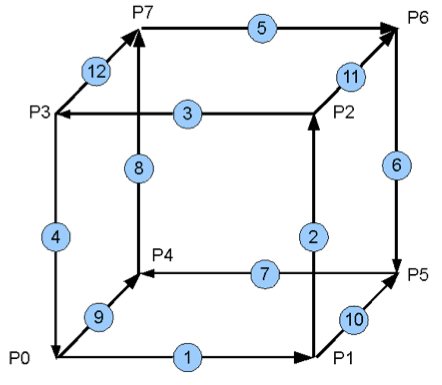
\includegraphics{lab5Cubic.png}


In the field of Image Processing filtering  especially for the use of noise reduction is used to remove unwanted noise, i.e., removing the noise of image sensors to further improve the analysis and processing of the image. Denoising of image traditionally employees a Gaussian filtering technique. This smooths the image over a local region thus removing any noise present. Smaller structures present in the image are completely lost but structures that are more coarser would still be present. We can see formulate the Gaussian filtering as convolution between the image and a Gaussian Kernel as shown below.

$$I_{output} = I_{Input}* h(x,y)$$
where $h(x,y)$ is the Gaussian kernel defined as  

$$h(x,y) = \frac{1}{{2\pi}\sigma^2}e^{-\frac{x^2+y^2}{2\sigma^2}}$$

where $\sigma$ gives the variance of the Gaussian that determines the degree of blurring or smoothing.

Below we can see a discrete example of Gaussian filtering of an image where the values of the image is just a mean of images around it that is processed in $x$ and $y$ direction separately.
$$ \frac{1}{4}
\begin{bmatrix} 
    1 \\ 2 \\ 1  
\end{bmatrix} 
*
\frac{1}{4}
\begin{bmatrix} 
    1 & 2 & 1
\end{bmatrix} = \frac{1}{16}
\begin{bmatrix} 
    1 & 2 & 1 \\ 
    2 & 4 & 2 \\
    1 & 2 & 1
\end{bmatrix} $$

We can clearly see that these traditional techniques do not care about the edges and this information is degraded when applying such methods.
\section{Bilateral Filtering}
Bilateral filtering is a non linear filtering that preserves strong edges. This primarily work for bilateral filtering was done by Aurich et al 1995 who worked on nonlinear Gaussian filters. This was later refined and was called as Bilateral filter by Tomasi et al. Unlike traditional filtering process where the filtering is done by replacing the pixel value by average values of pixel around it, it also 	accounts for the pixel intensities around it while performing filtering. This produces a filtering process that uses the domain and range data of an image to produce images where the edge information is retained.

The filter can be defined as below
$$ I^\text{filtered}(x) = \frac{1}{W_p} \sum_{x_i \in \Omega} I(x_i)f_r(\|I(x_i)-I(x)\|)g_s(\|x_i-x\|)$$

where the weight $W_{p}$ is defined as 
$$ W_p = \sum_{x_i \in \Omega}{f_r(\|I(x_i)-I(x)\|)g_s(\|x_i-x\|)} $$

Here $I^{Filtered}$ is output image that is filtered.   $I$ is the input image and $x$ is the location of the current pixel.	$\omega$ is the window centered at $x$ where the operation takes place. $f_{r}$ and $g_{s}$ are defined as the range and the spatial kernel receptively to smooth the image according to its intensity and coordinate. A visual overview of the process can beem seen below where all the parameters have been visualized.

\begin{figure}[ht!]
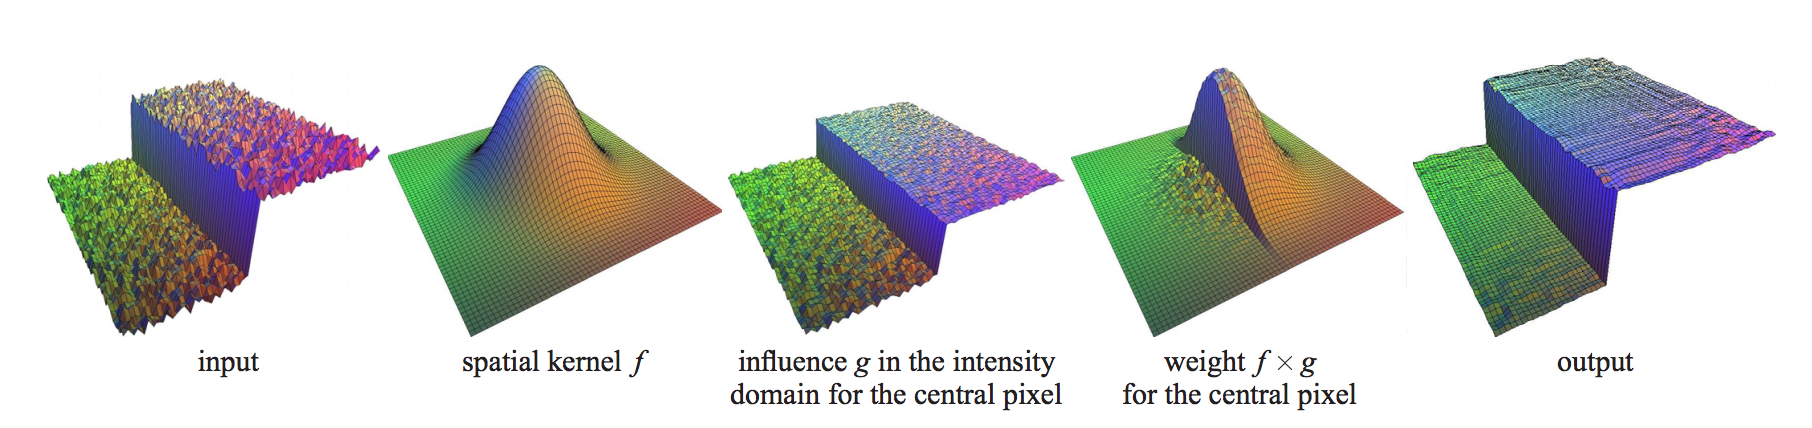
\includegraphics[scale=0.24]{Overall.png}
\caption{The complete process visualized}
\end{figure}

This approach has a lot of application such as Denoising, Contrast Management, Depth Reconstruction, Data Fusion and demosaicking.	

The salient feature of this method is that its formulation is very simple as each of the pixel values are a weighted mean of the negligible and this can be tuned with just 2 parameters that tell us the spatial size and the range to get the desired output. With the advent for new algorithm it can be used also in a non iterative manner  and at a faster speed making it even real time.

	

\section{Matlab Implementation}
In this project I used the implementation of the famous paper - "Bilateral Filtering for Gray and Color Images" by C. Tomasi et al. In this report you find the study of the paper, the code and analysis. Implementation includes bilateral filter for both color and gray images, image abstraction - cartoonizing the image and demo scripts to prepare this report. 

\section{Application and Results}
In this section we discuss the 2 major application of such filtering techniques that we have developed, They are denoising and image abstraction. The denoising was done for both color and gray-scale image and image abstraction was done for color only. First we test the algorithm with synthetic image of a check-board where the noise was added. 


\begin{figure}[ht!]
        \centering
                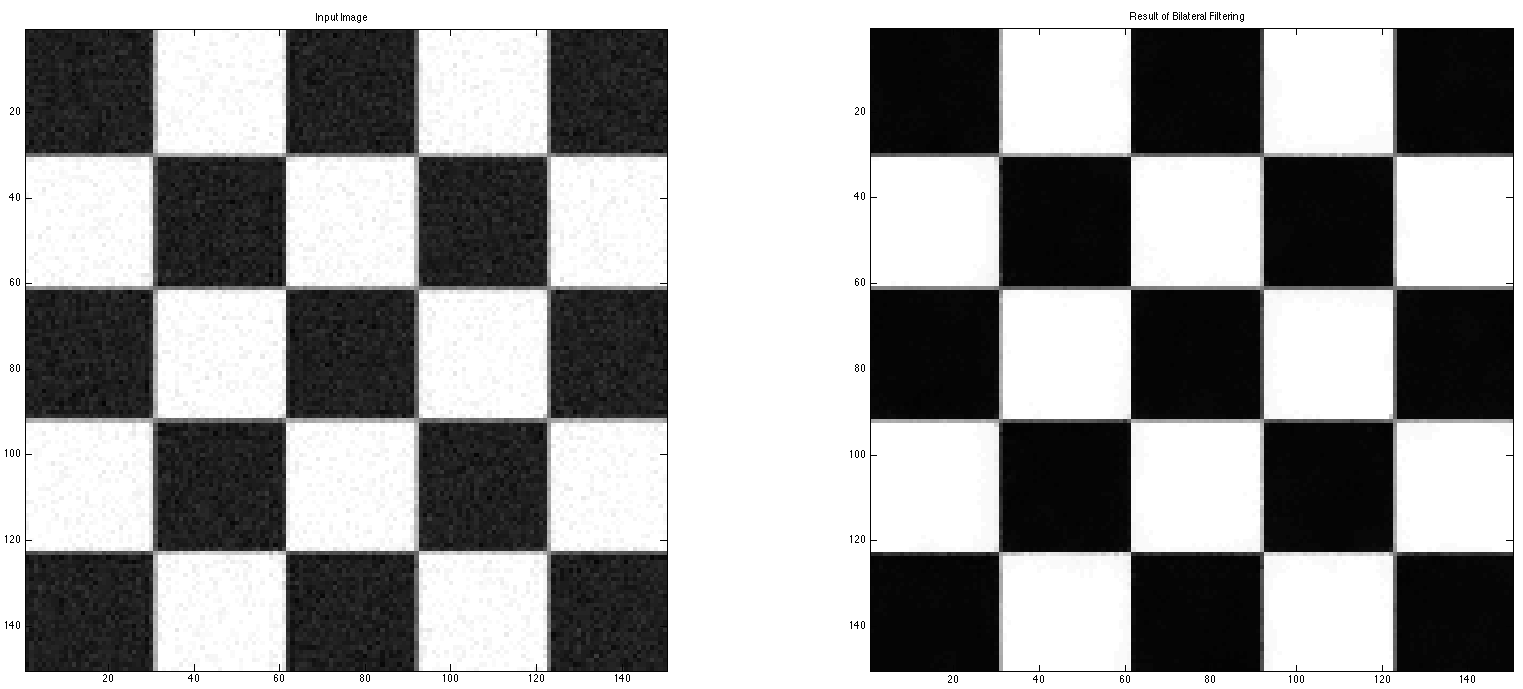
\includegraphics[width=\textwidth]{syn1}
                \caption{Denoising for synthetic Image}
\end{figure}

Here we can see that the denoising for gray-level image is very well performed. Most of the major edges are preserved while removing all the noise that was added. It is similar for color image with the addition that there is no phantom colors introduced during the step.  There is definitely a loss in texture but that is expected from any denosing application in Image processing.


\begin{figure}[ht!]
        \centering
                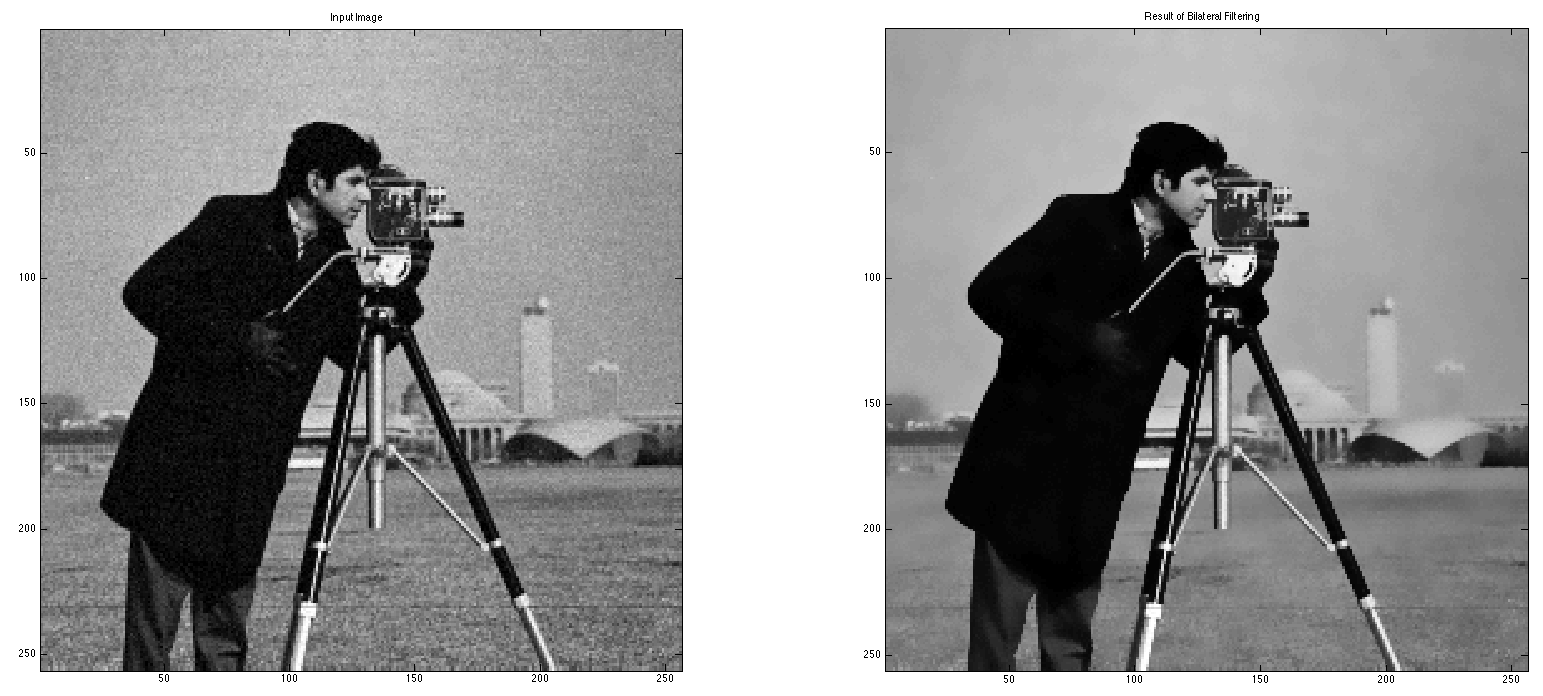
\includegraphics[width=\textwidth]{bw1}
                \caption{Denoising for gray-scale Image}
\end{figure}

\begin{figure}[ht!]
        \centering
                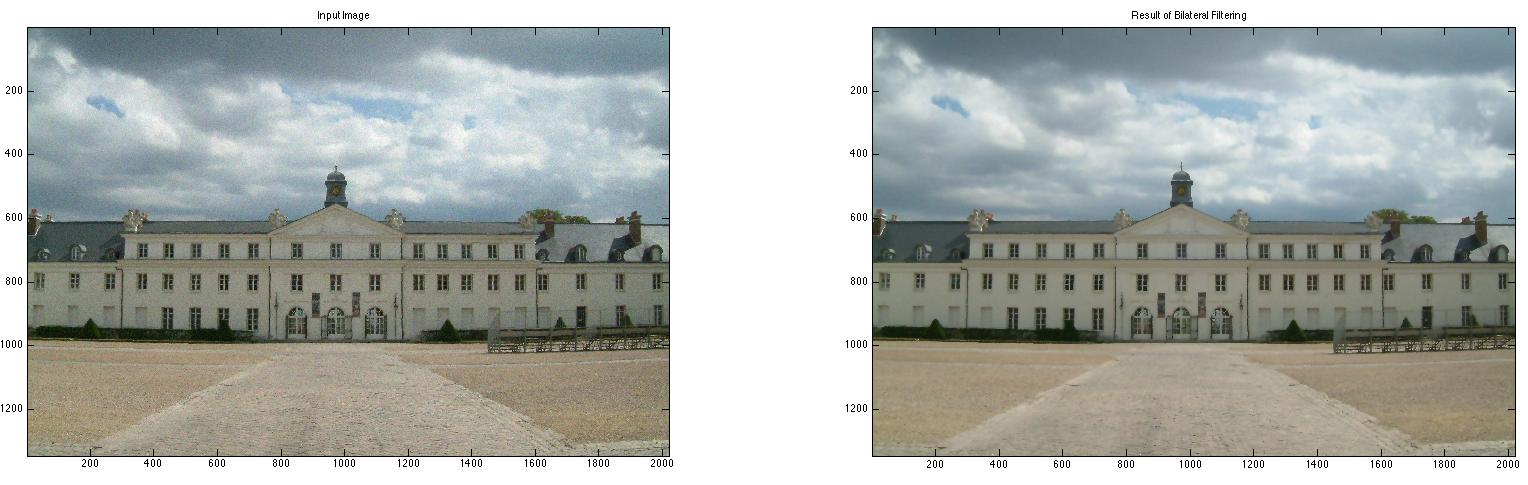
\includegraphics[width=\textwidth]{color1}
                \caption{Denoising for color Image}
\end{figure}

Image abstraction was done using the idea provided by Winnemoller et al. This can be viewed as another application of bilateral filtering.

\begin{figure}[ht!]
        \centering
        \begin{subfigure}[b]{0.45\textwidth}
                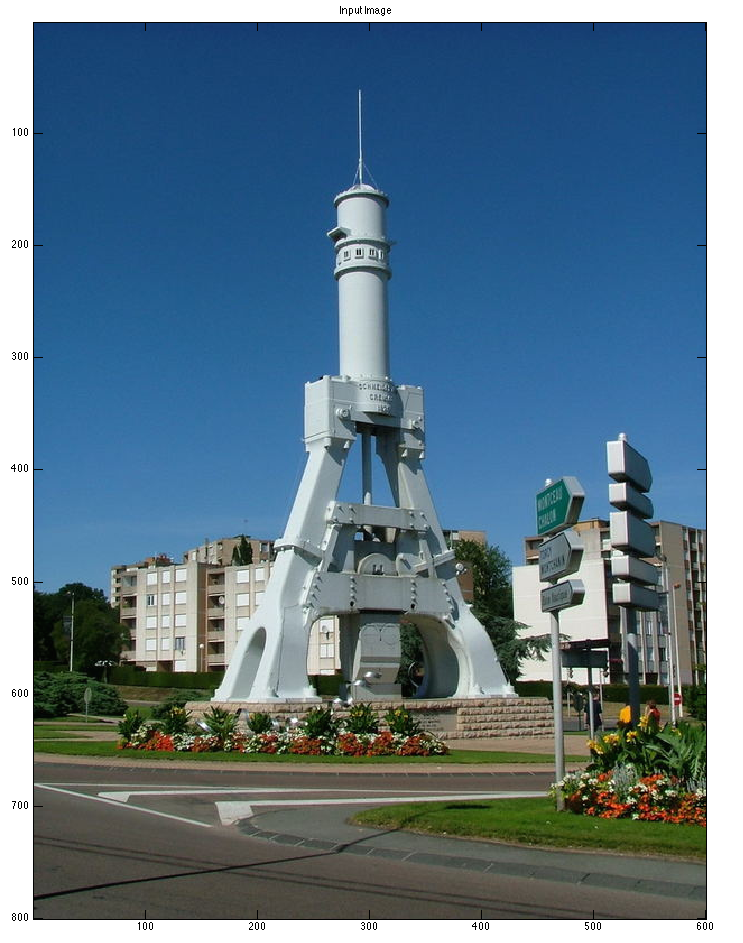
\includegraphics[width=\textwidth]{e1}
                \caption{Original Image}
        \end{subfigure}%
        ~ 
        \begin{subfigure}[b]{0.45\textwidth}
                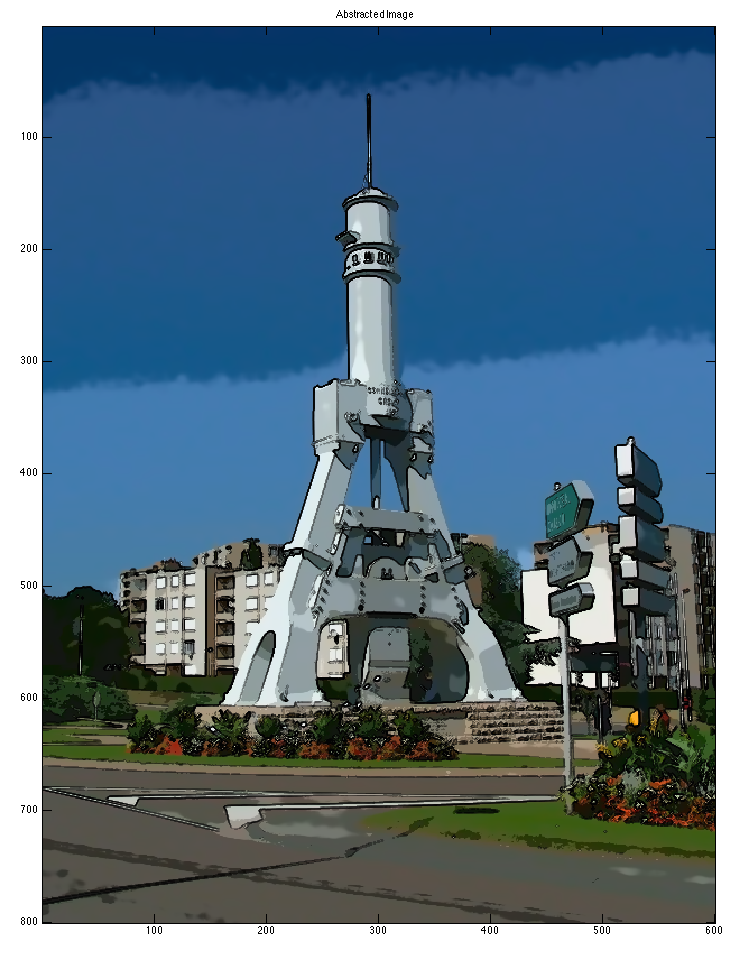
\includegraphics[width=\textwidth]{ae1}
                \caption{Abstracted Image}
        \end{subfigure}
        \caption{Image Abstraction}
\end{figure}
\pagebreak

Here below we can see the parameter changes effecting on the cameraman image. There are two parameters we experimented: $w$ - window size and $\sigma$ - standard deviation.

\begin{figure}[ht!]
        \centering
        
        \begin{subfigure}[b]{0.45\textwidth}
                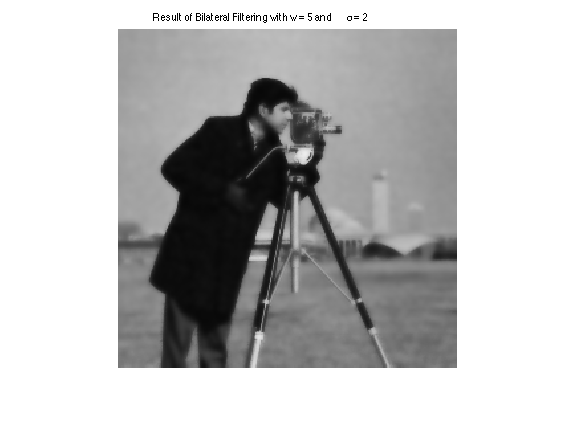
\includegraphics[width=\textwidth]{w5s2.png}
                \caption{w = 5, $\sigma$ = 2}
        \end{subfigure}%
        \begin{subfigure}[b]{0.45\textwidth}
                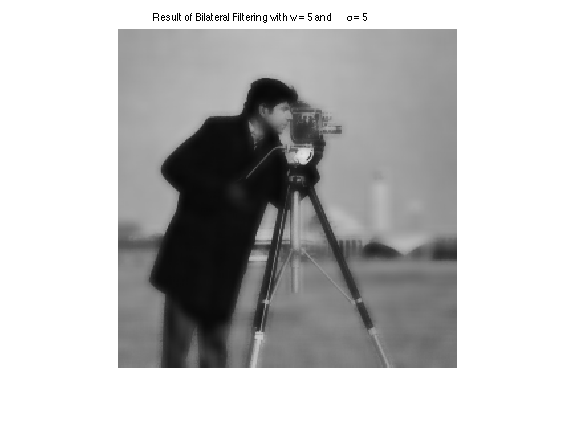
\includegraphics[width=\textwidth]{w5s5.png}
                \caption{w = 5, $\sigma$ = 5}
        \end{subfigure}
        
        \begin{subfigure}[b]{0.45\textwidth}
                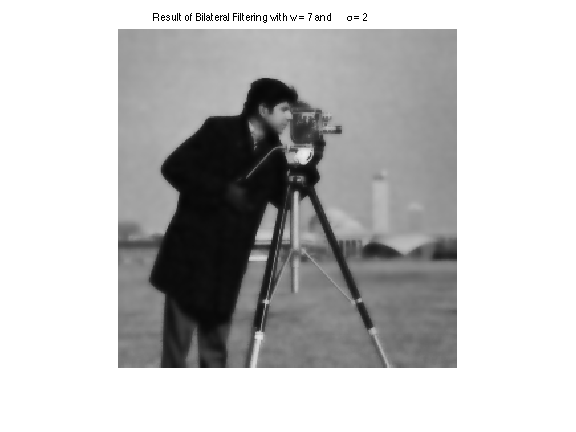
\includegraphics[width=\textwidth]{w7s2.png}
                \caption{w = 7, $\sigma$ = 2}
        \end{subfigure}%
        \begin{subfigure}[b]{0.45\textwidth}
                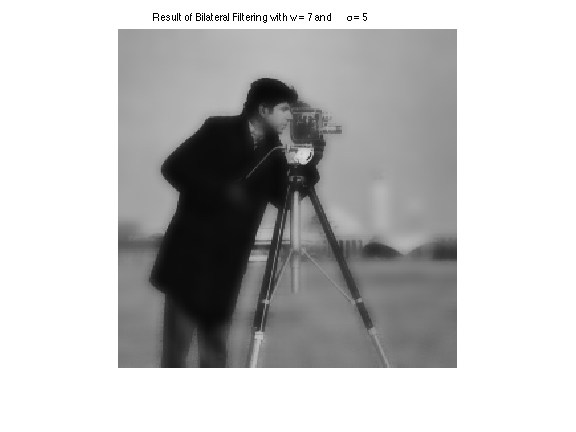
\includegraphics[width=\textwidth]{w7s5.png}
                \caption{w = 7, $\sigma$ = 5}
        \end{subfigure}
        
        \begin{subfigure}[b]{0.45\textwidth}
                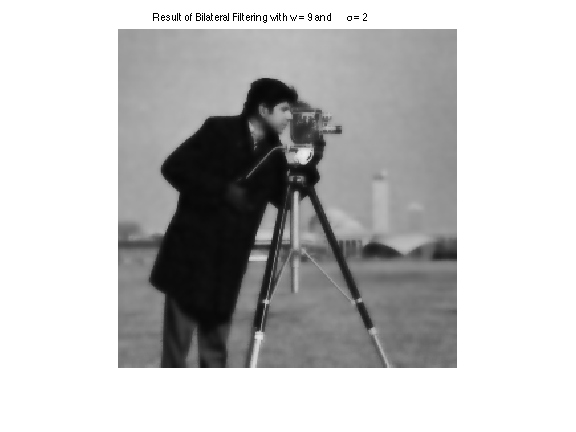
\includegraphics[width=\textwidth]{w9s2.png}
                \caption{w = 9, $\sigma$ = 2}
        \end{subfigure}%
        \begin{subfigure}[b]{0.45\textwidth}
                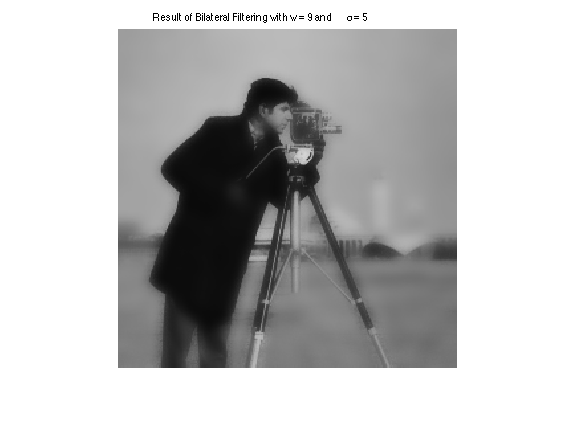
\includegraphics[width=\textwidth]{w9s5.png}
                \caption{w = 9, $\sigma$ = 5}
        \end{subfigure}
        \caption{Cameraman Image}
\end{figure}

\pagebreak


\section{Conclusion}
We conclude that bilateral filtering is very simple and elegant algorithm image denoising that preserves edges. This was achieved by the addition of intensity range term to classical image filtering algorithm produce the desired result. The range and the spatial coefficients could be varied accordingly to use for any specific application. In future work we could focus on making this algorithm more efficient as currently it take $O(n^{2})$ time to filter an image.

\end{document}


